% !TEX TS-program = pdflatex
% !TEX encoding = UTF-8 Unicode

% This is a simple template for a LaTeX document using the "article" class.
% See "book", "report", "letter" for other types of document.

\documentclass[11pt]{paper} % use larger type; default would be 10pt

%%% Examples of Article customizations
% These packages are optional, depending whether you want the features they provide.
% See the LaTeX Companion or other references for full information.

%%% PAGE DIMENSIONS
%\usepackage{geometry} % to change the page dimensions
%\geometry{a4paper} % or letterpaper (US) or a5paper or....
% \geometry{margin=2in} % for example, change the margins to 2 inches all round
% \geometry{landscape} % set up the page for landscape
%   read geometry.pdf for detailed page layout information
\usepackage{mathtools}
\usepackage{graphicx} % support the \includegraphics command and options

% \usepackage[parfill]{parskip} % Activate to begin paragraphs with an empty line rather than an indent

%%% PACKAGES
%\usepackage{booktabs} % for much better looking tables
%\usepackage{array} % for better arrays (eg matrices) in maths
%\usepackage{paralist} % very flexible & customisable lists (eg. enumerate/itemize, etc.)
%\usepackage{verbatim} % adds environment for commenting out blocks of text & for better verbatim
%\usepackage{subfig} % make it possible to include more than one captioned figure/table in a single float
% These packages are all incorporated in the memoir class to one degree or another...

%%% HEADERS & FOOTERS
%\usepackage{fancyhdr} % This should be set AFTER setting up the page geometry
%\pagestyle{fancy} % options: empty , plain , fancy
%\renewcommand{\headrulewidth}{0pt} % customise the layout...
%\lhead{}\chead{}\rhead{}
%\lfoot{}\cfoot{\thepage}\rfoot{}

%%% SECTION TITLE APPEARANCE
%\usepackage{sectsty}
%\allsectionsfont{\sffamily\mdseries\upshape} % (See the fntguide.pdf for font help)
% (This matches ConTeXt defaults)

%%% ToC (table of contents) APPEARANCE
%\usepackage[nottoc,notlof,notlot]{tocbibind} % Put the bibliography in the ToC
%\usepackage[titles,subfigure]{tocloft} % Alter the style of the Table of Contents
%\renewcommand{\cftsecfont}{\rmfamily\mdseries\upshape}
%\renewcommand{\cftsecpagefont}{\rmfamily\mdseries\upshape} % No bold!

%%% END Article customizations

%%% The "real" document content comes below...

\title{Infering the volume of binding pocket of odor-receptors in Drosophila from the neural data}
\author{Majid Saberi \and Hamed Seyed-allaei\thanks{hamed@ipm.ir}}
\institution{School of Cognitive Science, Institute for Research in Fundamental Sciences (IPM), \\Tehran, Iran}
%\date{} % Activate to display a given date or no date (if empty),
         % otherwise the current date is printed 


\begin{document}
\maketitle
\begin{abstract}
To be writen later.
\end{abstract}

\section{Introduction}

\section{Methods}
A receptor neuron $n$ is excited by odorants $m \in M_n$ and the response of $r_{nm}$ is recorded, where $0 \le r_{nm} \le 1$. 
Different neurons might be excited by different set of odorants $M_n$. 
The response $r_{nm}$ depends on the molecular volume of the odorant, $v_m$, 
and many other possible physio-chemical properties of the molecule $m$; 
Therefore, we separate the response $r_{nm}$ into two terms:
\begin{equation}
r_{nm} = f_n(v_m) \psi_{nm}.
\label{eqn:factors}
\end{equation}
The first term, $f_n(v)$, depends only on the molecular volume of odorants.
The second term, $\psi_{nm}$ may include every other properties of molecules, but the molecular volume.
Both terms are characteristic of each receptor, and they might vary from neuron to neuron.
In fact, the first term, $f_n(v)$, is the tuning curve of neuron $n$ in respect to the feature of molecular volumes, 
and like many other tuning curves, it can be approximated with a Gaussian function
\begin{equation}
\displaystyle f_n(v) = e^{-\frac{(v-v_n)^2}{2\sigma^2_n}}, 
\end{equation}
where, $v_n$ is the preferred molecular volume of receptor $n$ and $\sigma_n$ represents its volume selectivity. 
In this work we want to estimate $v_n$ and $\sigma_n$. 
To do so, first we calculate the response weighted average of molecular volumes, 
$\frac{\sum_{m\in M_n} v_m r_{nm}}{\sum_{m\in M_n} r_{nm}}$ and then we use equation \ref{eqn:factors}:
\begin{equation}
\frac{\displaystyle \sum_{m\in M_n} v_m r_{nm}}{\displaystyle \sum_{m\in M_n} r_{nm}} = \frac{\displaystyle \sum_{m\in M_n} v_m f_n(v_m) \psi_{nm}}{\displaystyle \sum_{m\in M_n} f_n(v_m) \psi_{nm}}.
\label{eqn:sta}
\end{equation}
Here we can convert $\sum$ to $\int$ following this rule:
\begin{equation}
\sum_{m\in M_n} \dots f_n(v_m) \psi_{nm} =  \langle \psi_{nm} \rangle_m \int_0^\infty \dots f_n(v) g_n(v)  dv. 
\label{eqn:sigma_to_int}
\end{equation}
In which, 
$\langle \psi_{nm} \rangle_m$ denotes the average of $\psi_{nm}$ over all $m \in M_n$, 
and can be moved out of the integral for it is independent of $v$.
In the above equation, 
$g_n(v)$ is the density of states, it says for each set of odorants $M_n$, how many molecules have a molecular volume in the range of $v$ and $v+dv$.
This function can be approximated by a Gaussian function of the form 
\begin{equation}
g_n(v) = e^{-\frac{(v- v_{M_n})^2}{2\sigma_{M_n}^2}},
\end{equation}
where $v_{M_n}$ and $\sigma_{M_n}$ are the average and standard deviation of molecular volume of the set $M_n$.
Now we convert $\sum$ to $\int$ in equation \ref{eqn:sta} using equation \ref{eqn:sigma_to_int}, to get
\begin{equation}
\frac{\displaystyle \sum_{m\in M_n} v_m r_{nm}}{\displaystyle \sum_{m\in M_n} r_{nm}} = \frac{\displaystyle \int v f_n(v) g_n(v) dv}{\displaystyle \int f_n(v) g_n(v) dv}.
\label{eqn:sta_int}
\end{equation}
We replace the product of $f_n(v)$ and $g_n(v)$ in the above equation with $h_n(v) = f_n(v) g_n(v)$, to make a simpler form
\begin{equation}
\frac{\displaystyle \sum_{m\in M_n} v_m r_{nm}}{\displaystyle \sum_{m\in M_n} r_{nm}} = \frac{\displaystyle \int_v v h_n(v) dv}{ \displaystyle \int_v  h_n(v) dv }.
\label{eqn:mean}
\end{equation}
The function $h_n(v)$ is a Gaussian function because it is the product of two Gaussian functions, 
\begin{equation}
h_n(v) = e^{-\frac{(v-\mu_{h_n})^2}{2\sigma_{h_n}^2}}, 
\end{equation}
so the right hand side of equation \ref{eqn:mean} is nothing but $\mu_{h_n}$. 
In a similar way, we can calculate $\sigma_{h_n}$ from the neural data.

We knew the mean $v_{M_n}$ and standard deviation $\sigma_{M_n}$ of $g_n(v)$ from the properties of the molecules. 
We just calculated the mean $\mu_{h_n}$ and standard deviation $\sigma_{h_n}$ of $h_n(v)$ from the neural data.
Now calculating the mean $v_n$ and the standard deviation $\sigma_n$ of $f_n(v)$ is trivial,
first we calculate $\sigma_n$ from 
\begin{equation}
\sigma_n^2 = \frac{\sigma^2_{g_n} \sigma^2_{h_n}}{\sigma^2_{g_n} - \sigma^2_{h_n}}
\end{equation}•
and then we calculate $v_n$ from 
\begin{equation}
v_n =  \sigma_n^2 \left ( \frac{\mu_{h_n}}{\sigma^2_{h_n}} - \frac{v_{g_n}}{\sigma^2_{g_n}} \right ).
\end{equation}•
The resulting $f_n(v)$ are plotted over the actual data, for one receptor (Fig.~\ref{fig:Or42a}) and for all (Fig.~\ref{fig:vol-res}).
Now we know the preferred volume $v_n$ of each receptor and also its volume selectivity $\sigma_n$.


\section{Results}


\begin{figure}
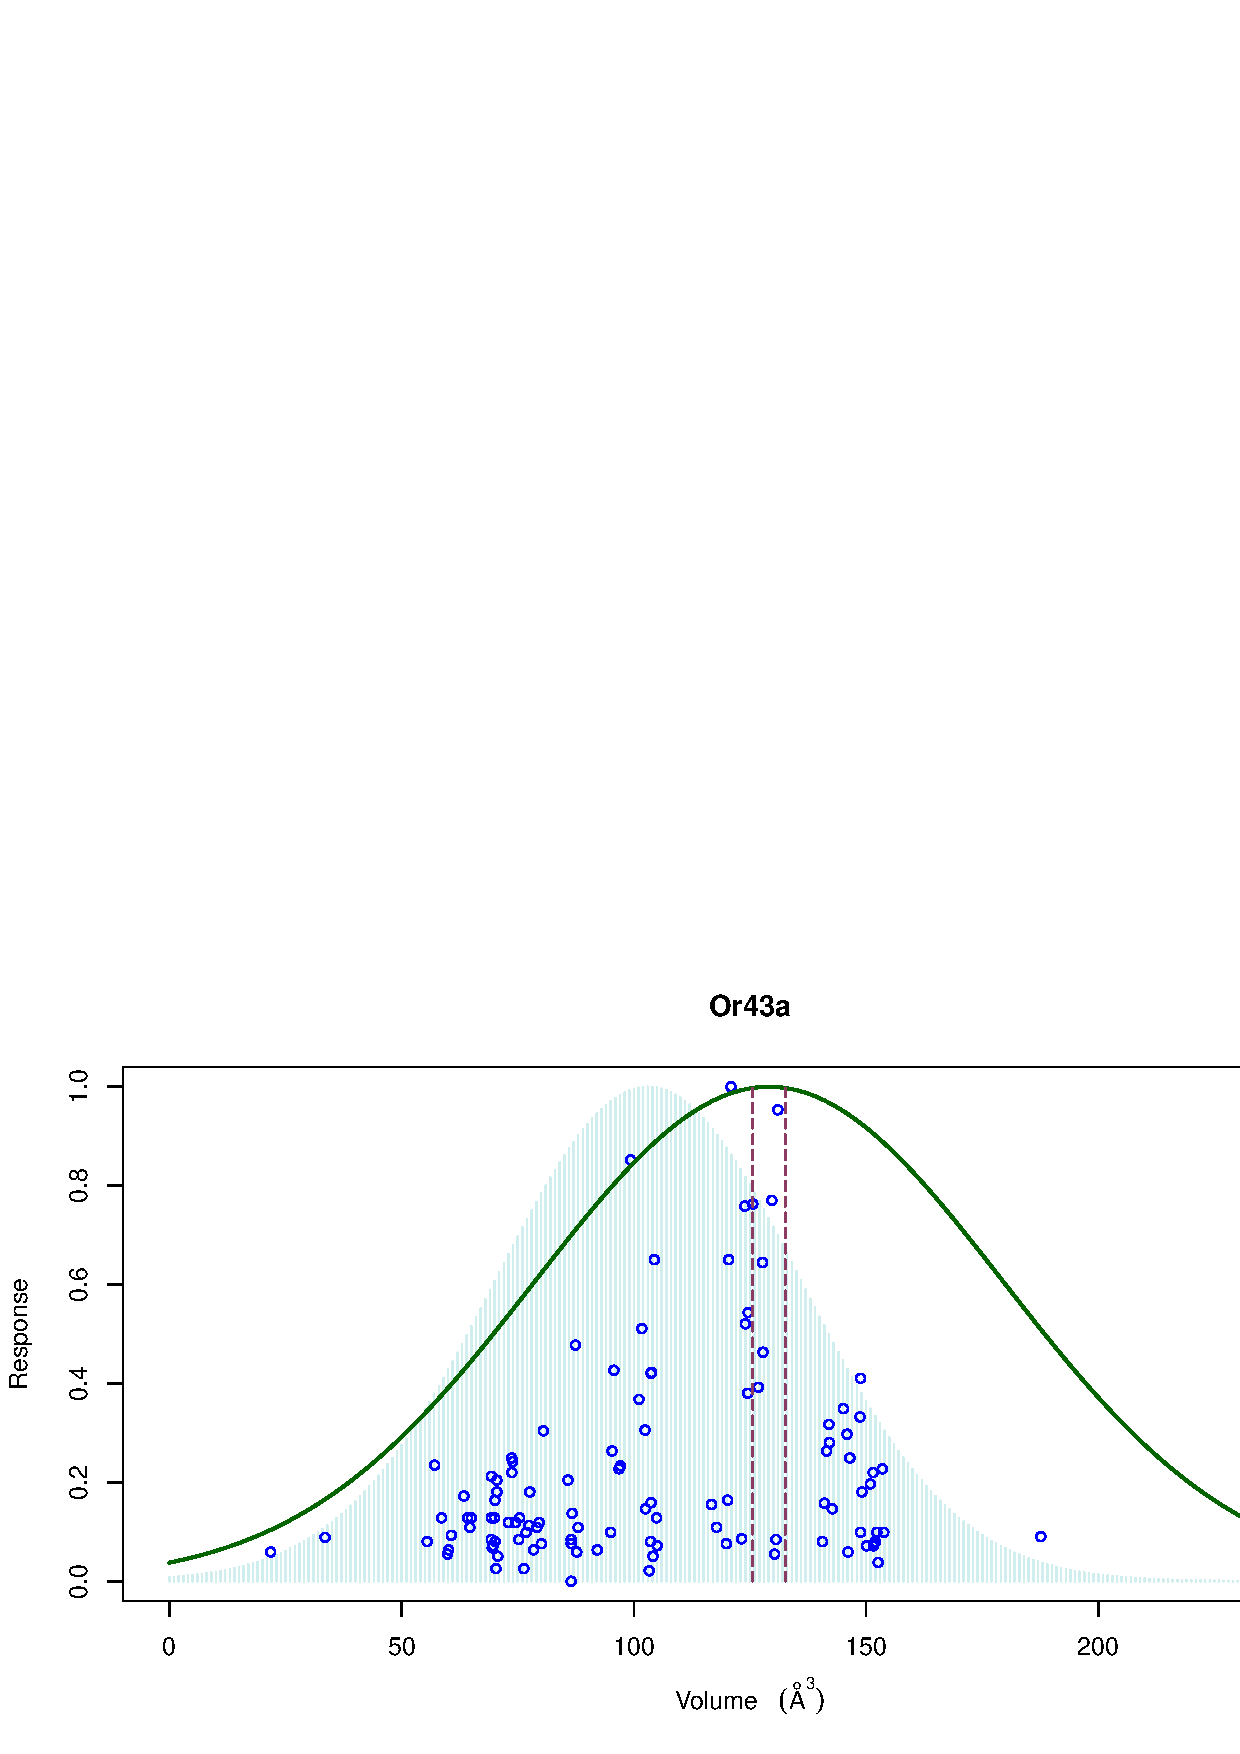
\includegraphics[width=\textwidth]{fig/vol-res-Or42a}
\caption{Response of an odor-receptor (Or42a) versus molecular volume of odorants.}
\label{fig:Or42a}
\end{figure}•

\begin{figure}
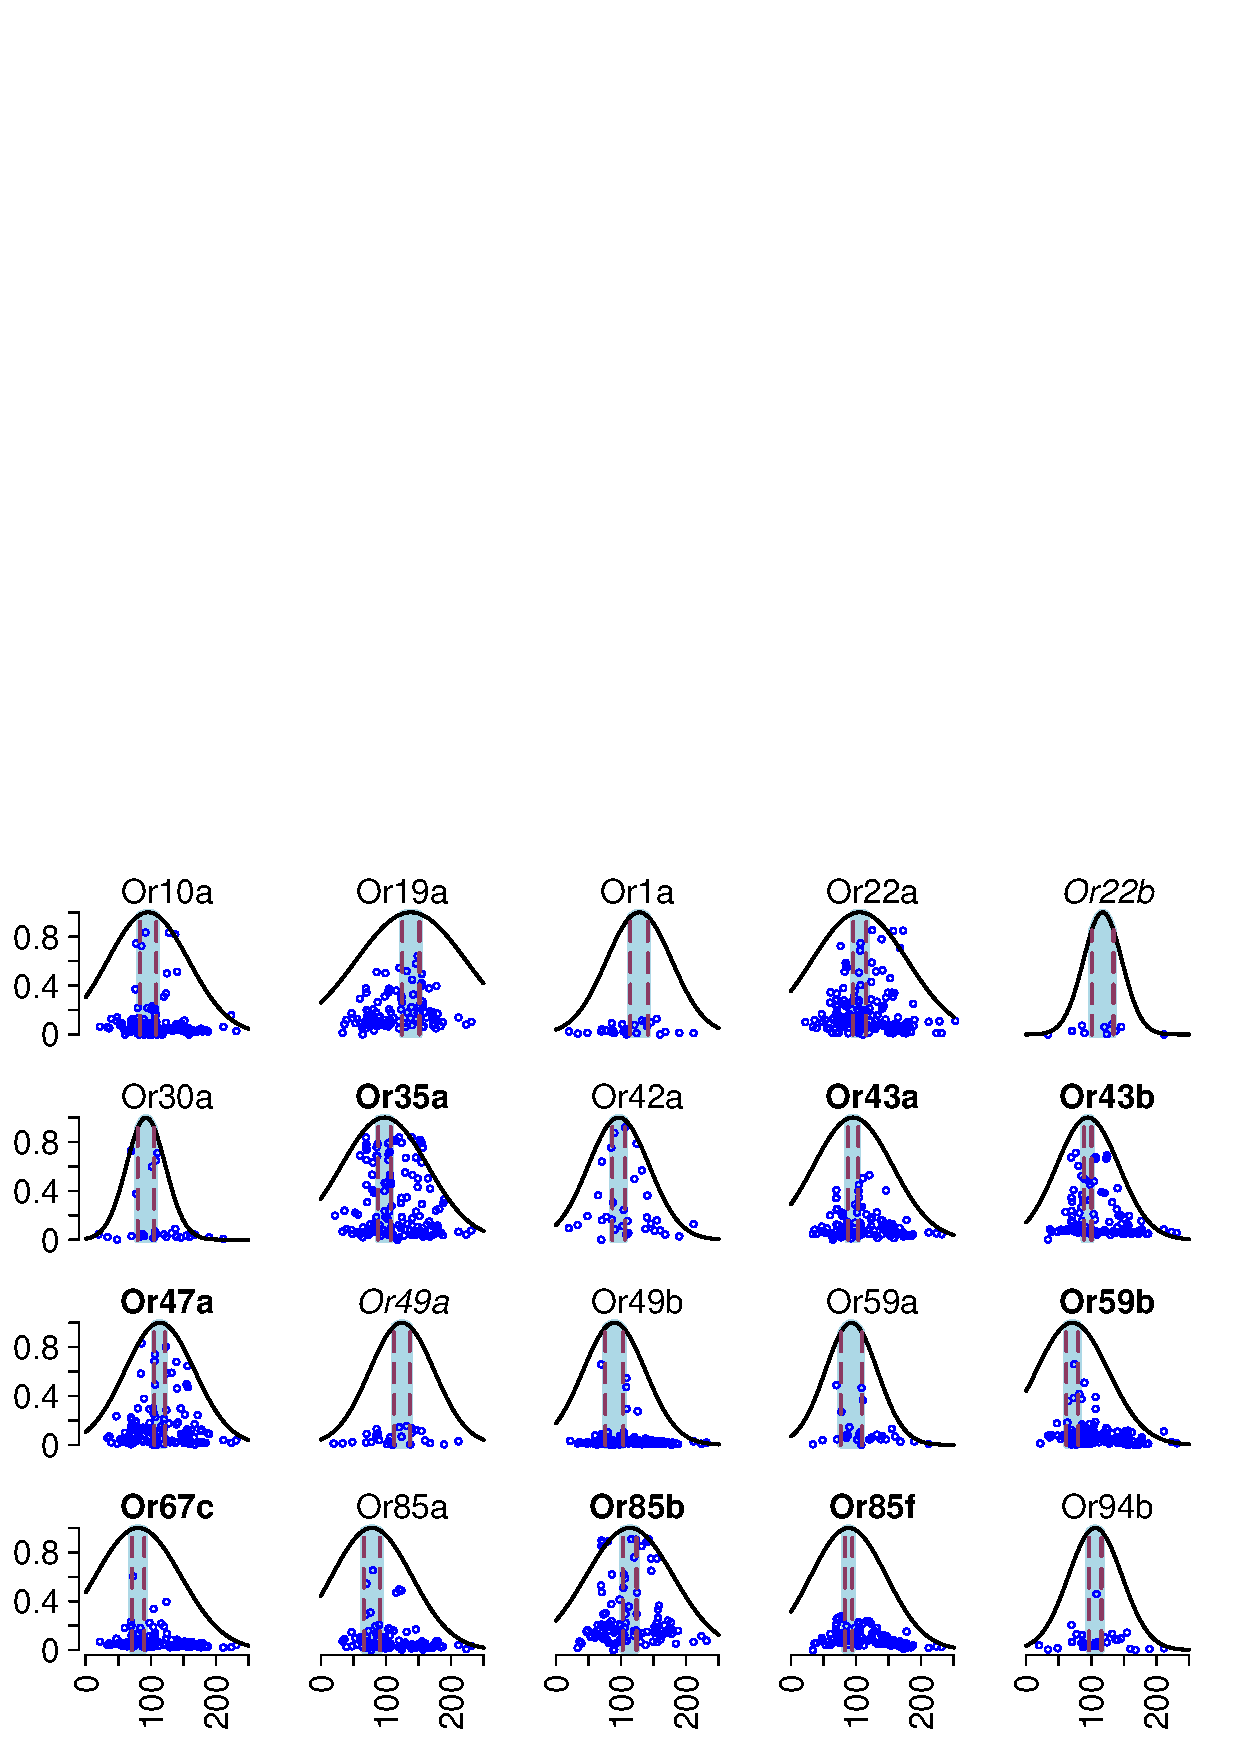
\includegraphics[width=\textwidth]{fig/vol-res}
\caption{Response of odor-receptors  versus molecular volume of odorants.}
\label{fig:vol-res}
\end{figure}•

\begin{figure}
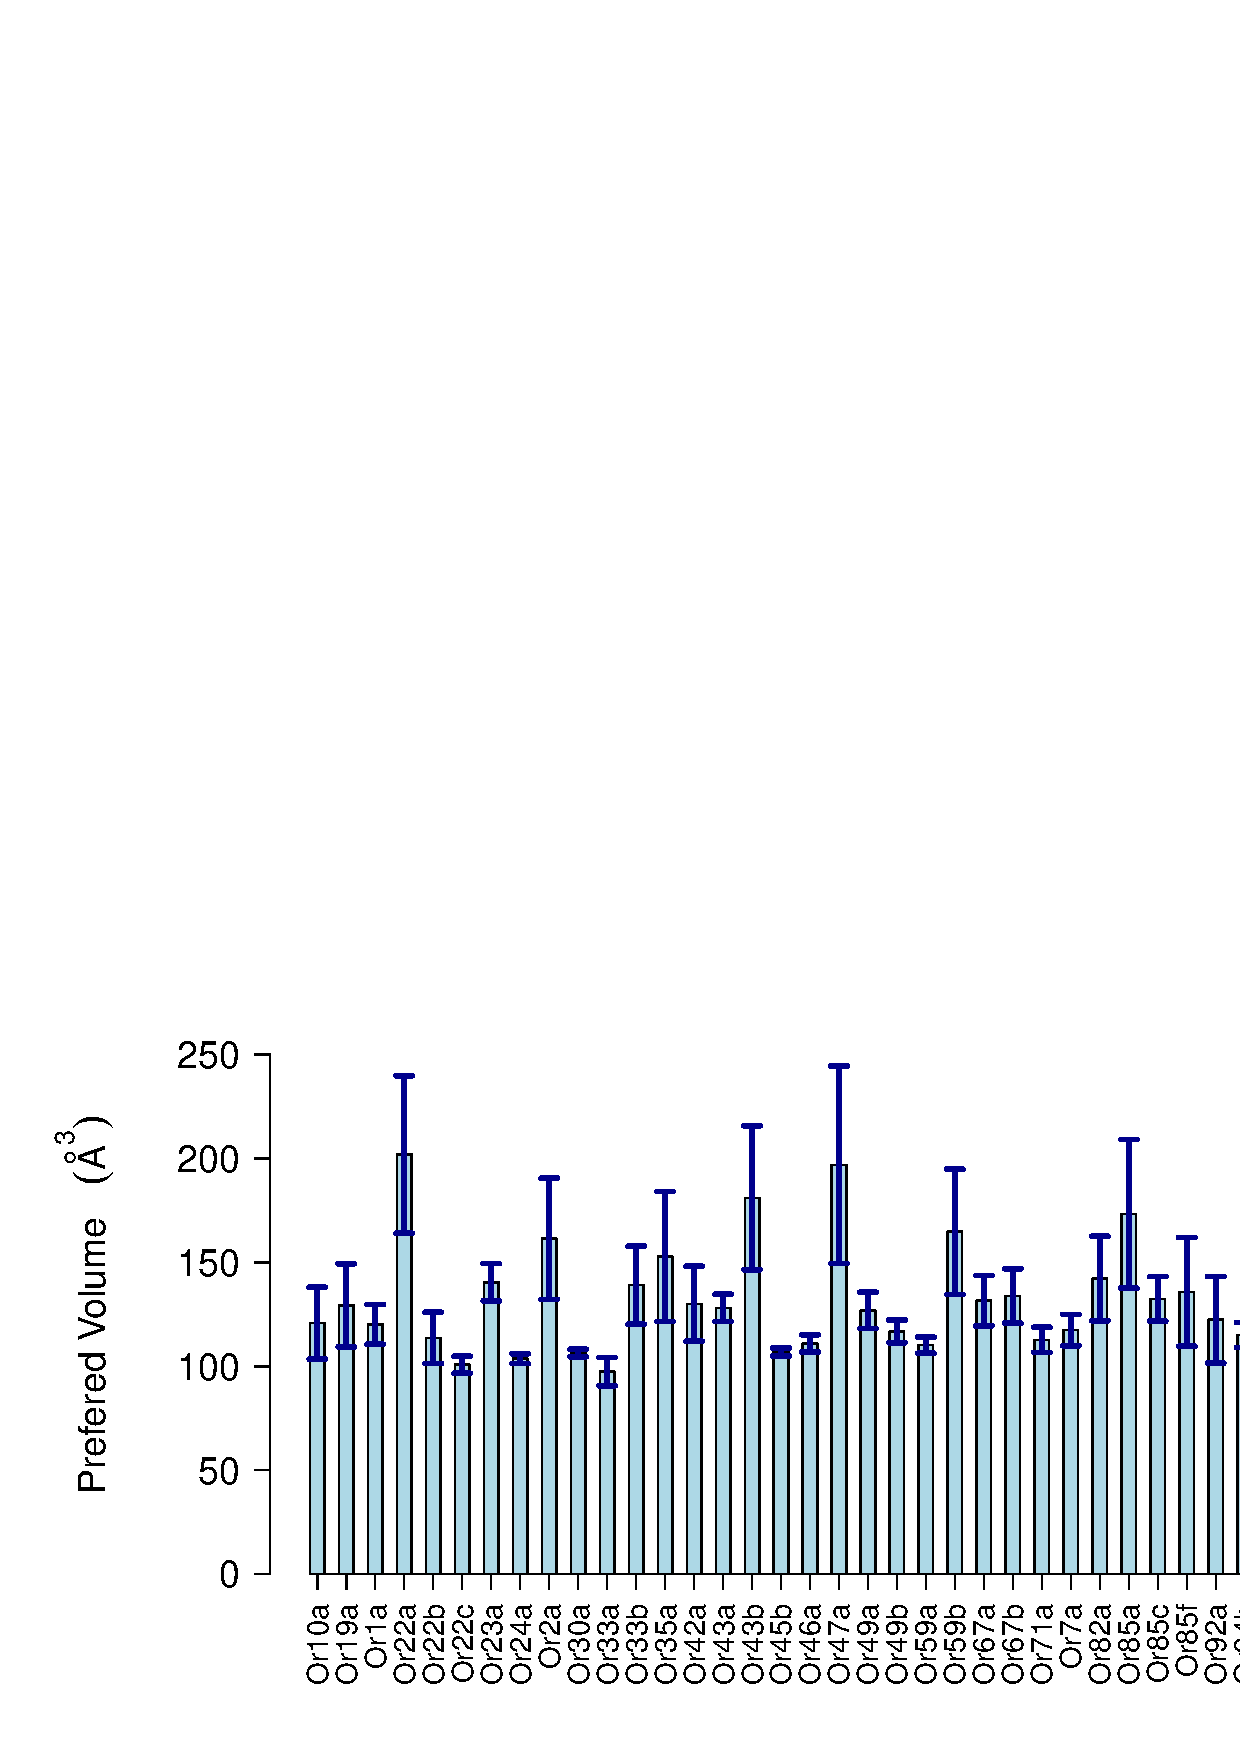
\includegraphics[width=\textwidth]{fig/mean-vol}
\caption{mean volume.}
\end{figure}•

\begin{figure}
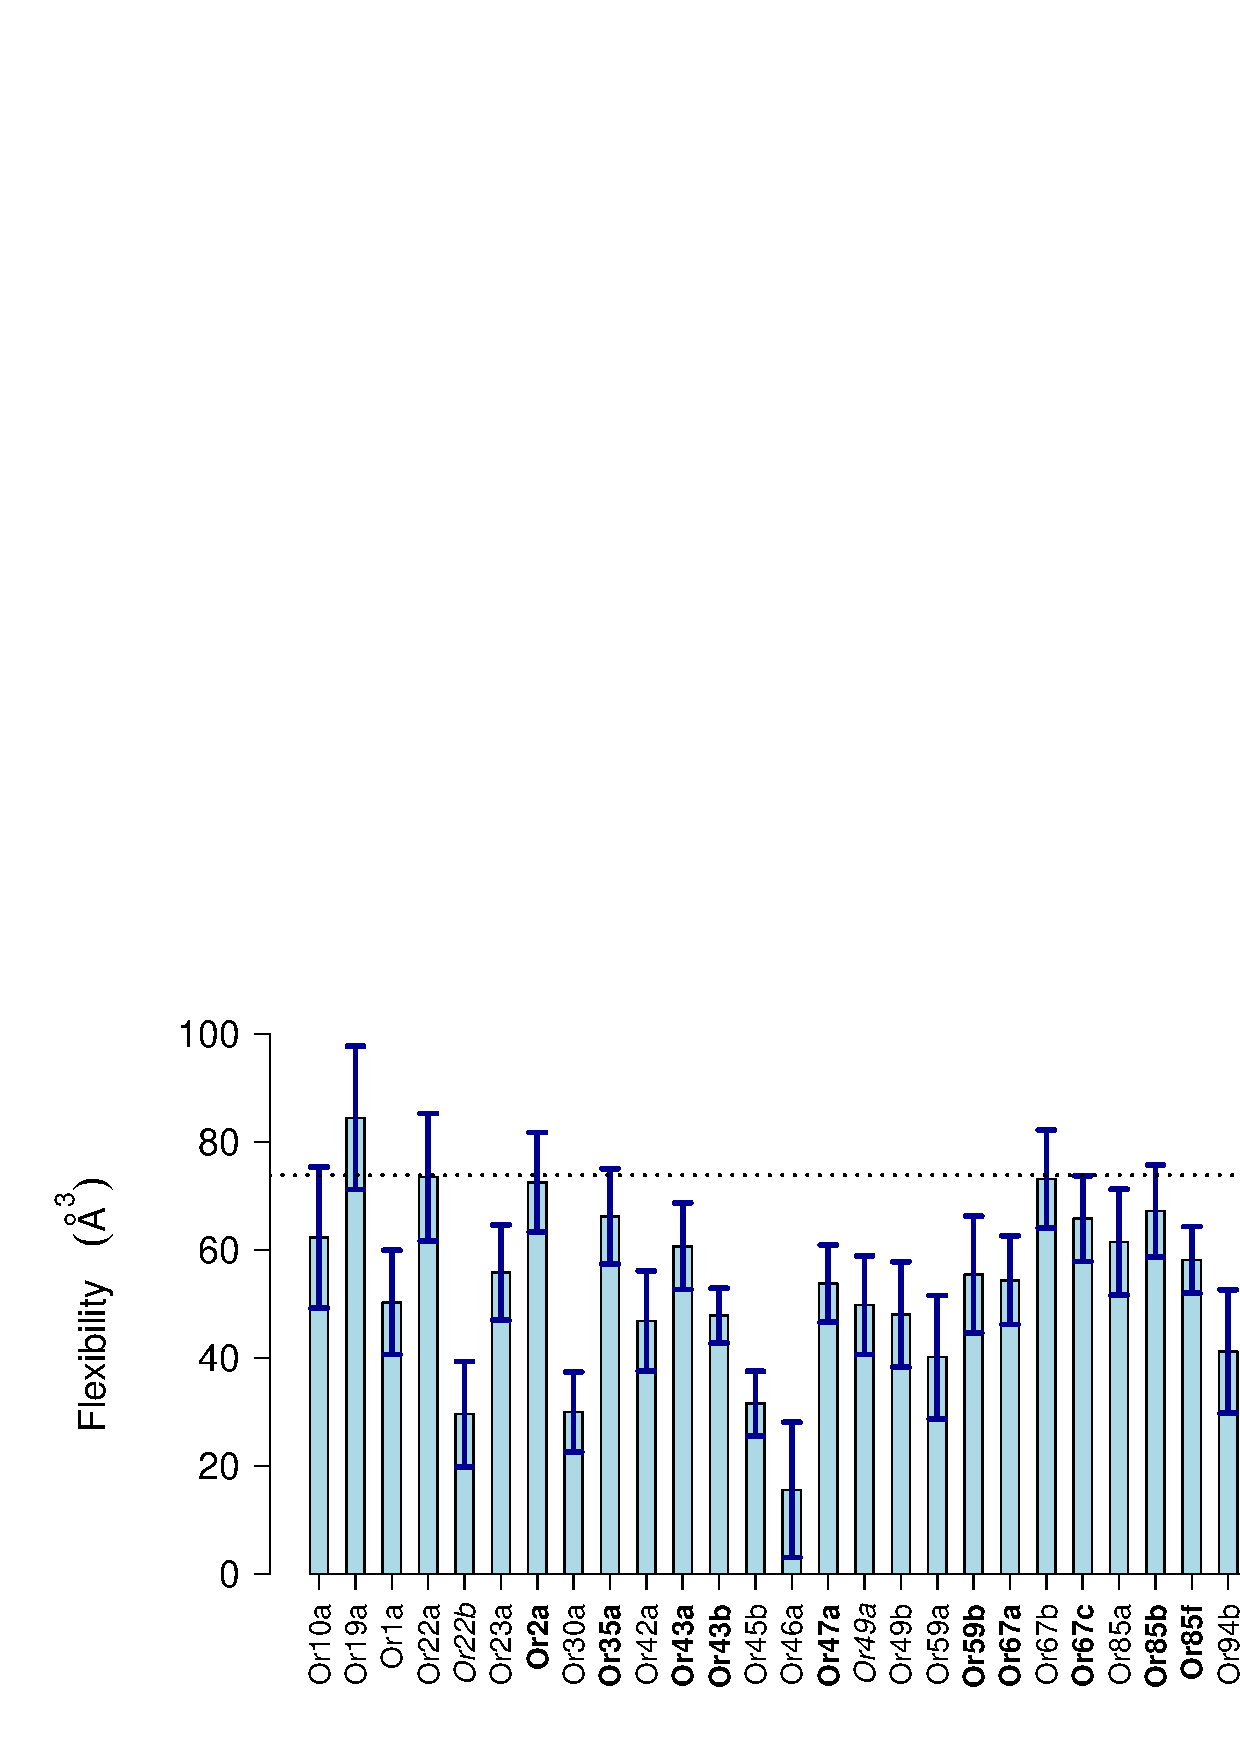
\includegraphics[width=\textwidth]{fig/std-vol}
\caption{std volume.}
\end{figure}•


\end{document}
